Como se nombró en el objetivo, se busca realizar el control de caudal o presión de un sistema hidráulico. Para esto fue necesario realizar la implementación de un banco de pruebas que cuente de tres partes (Figura \ref{fig:bancofull}).
\begin{itemize}
	\item Soporte para el motor y variador de velocidad al que se añadió 3 señales luminosas, llave selectora de dos puntos para seleccionar el modo de comunicación, llave selectora de tres puntos (encendido y sentido del motor) y un pulsador de parada de emergencia (Figura \ref{fig:banco}.a).

	Tanto el motor y los elementos adicionales fueron cableados (Figura \ref{fig:banco}.b) hacia las borneras del variador de velocidad y se tuvo en cuenta para esto las características y funciones del bornero de control proporcionado por el manual del variador de velocidad\cite{InstaManual}. 
	
	\item Soporte para una bomba en desuso de características no conocidas, con su bobinado quemado. Para facilitar el acople motor-bomba se mantuvo la carcasa y eje completo de la misma.
	\item Circuito hidráulico cerrado, que incluye un tanque, válvulas y sensores de caudal y presión.
\end{itemize}




\begin{figure}[htb]
	\centering
	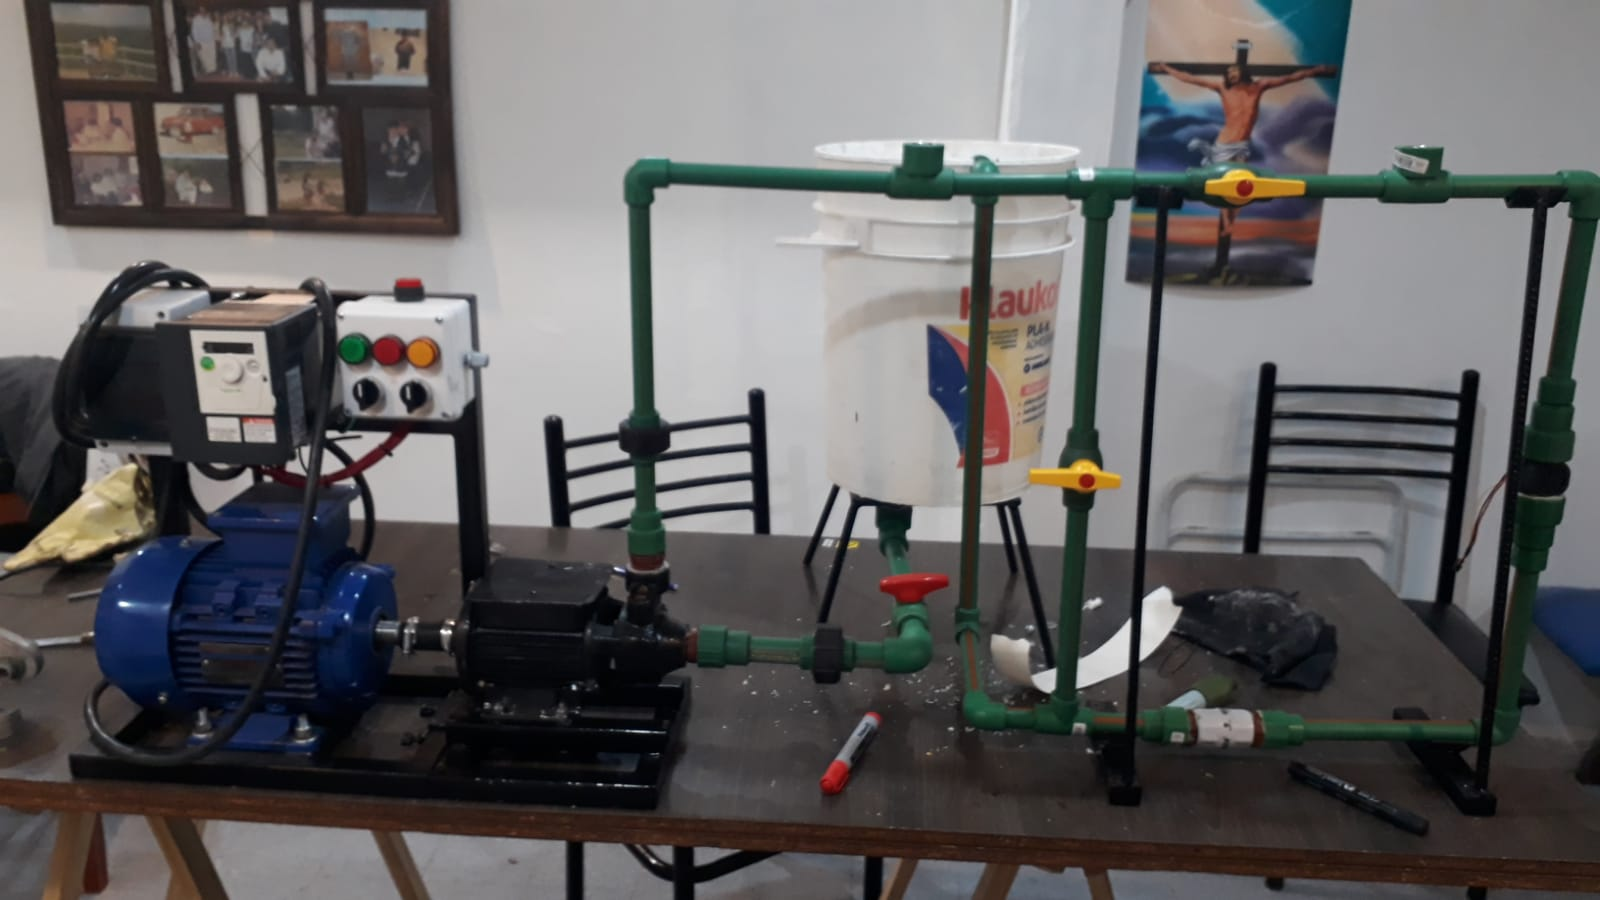
\includegraphics[width=0.9\linewidth]{bancofull.png}
	\captionof{figure}{Banco de pruebas completo}
	\label{fig:bancofull}
\end{figure}


\begin{figure}[H]
	\centering
	\subfigure[]{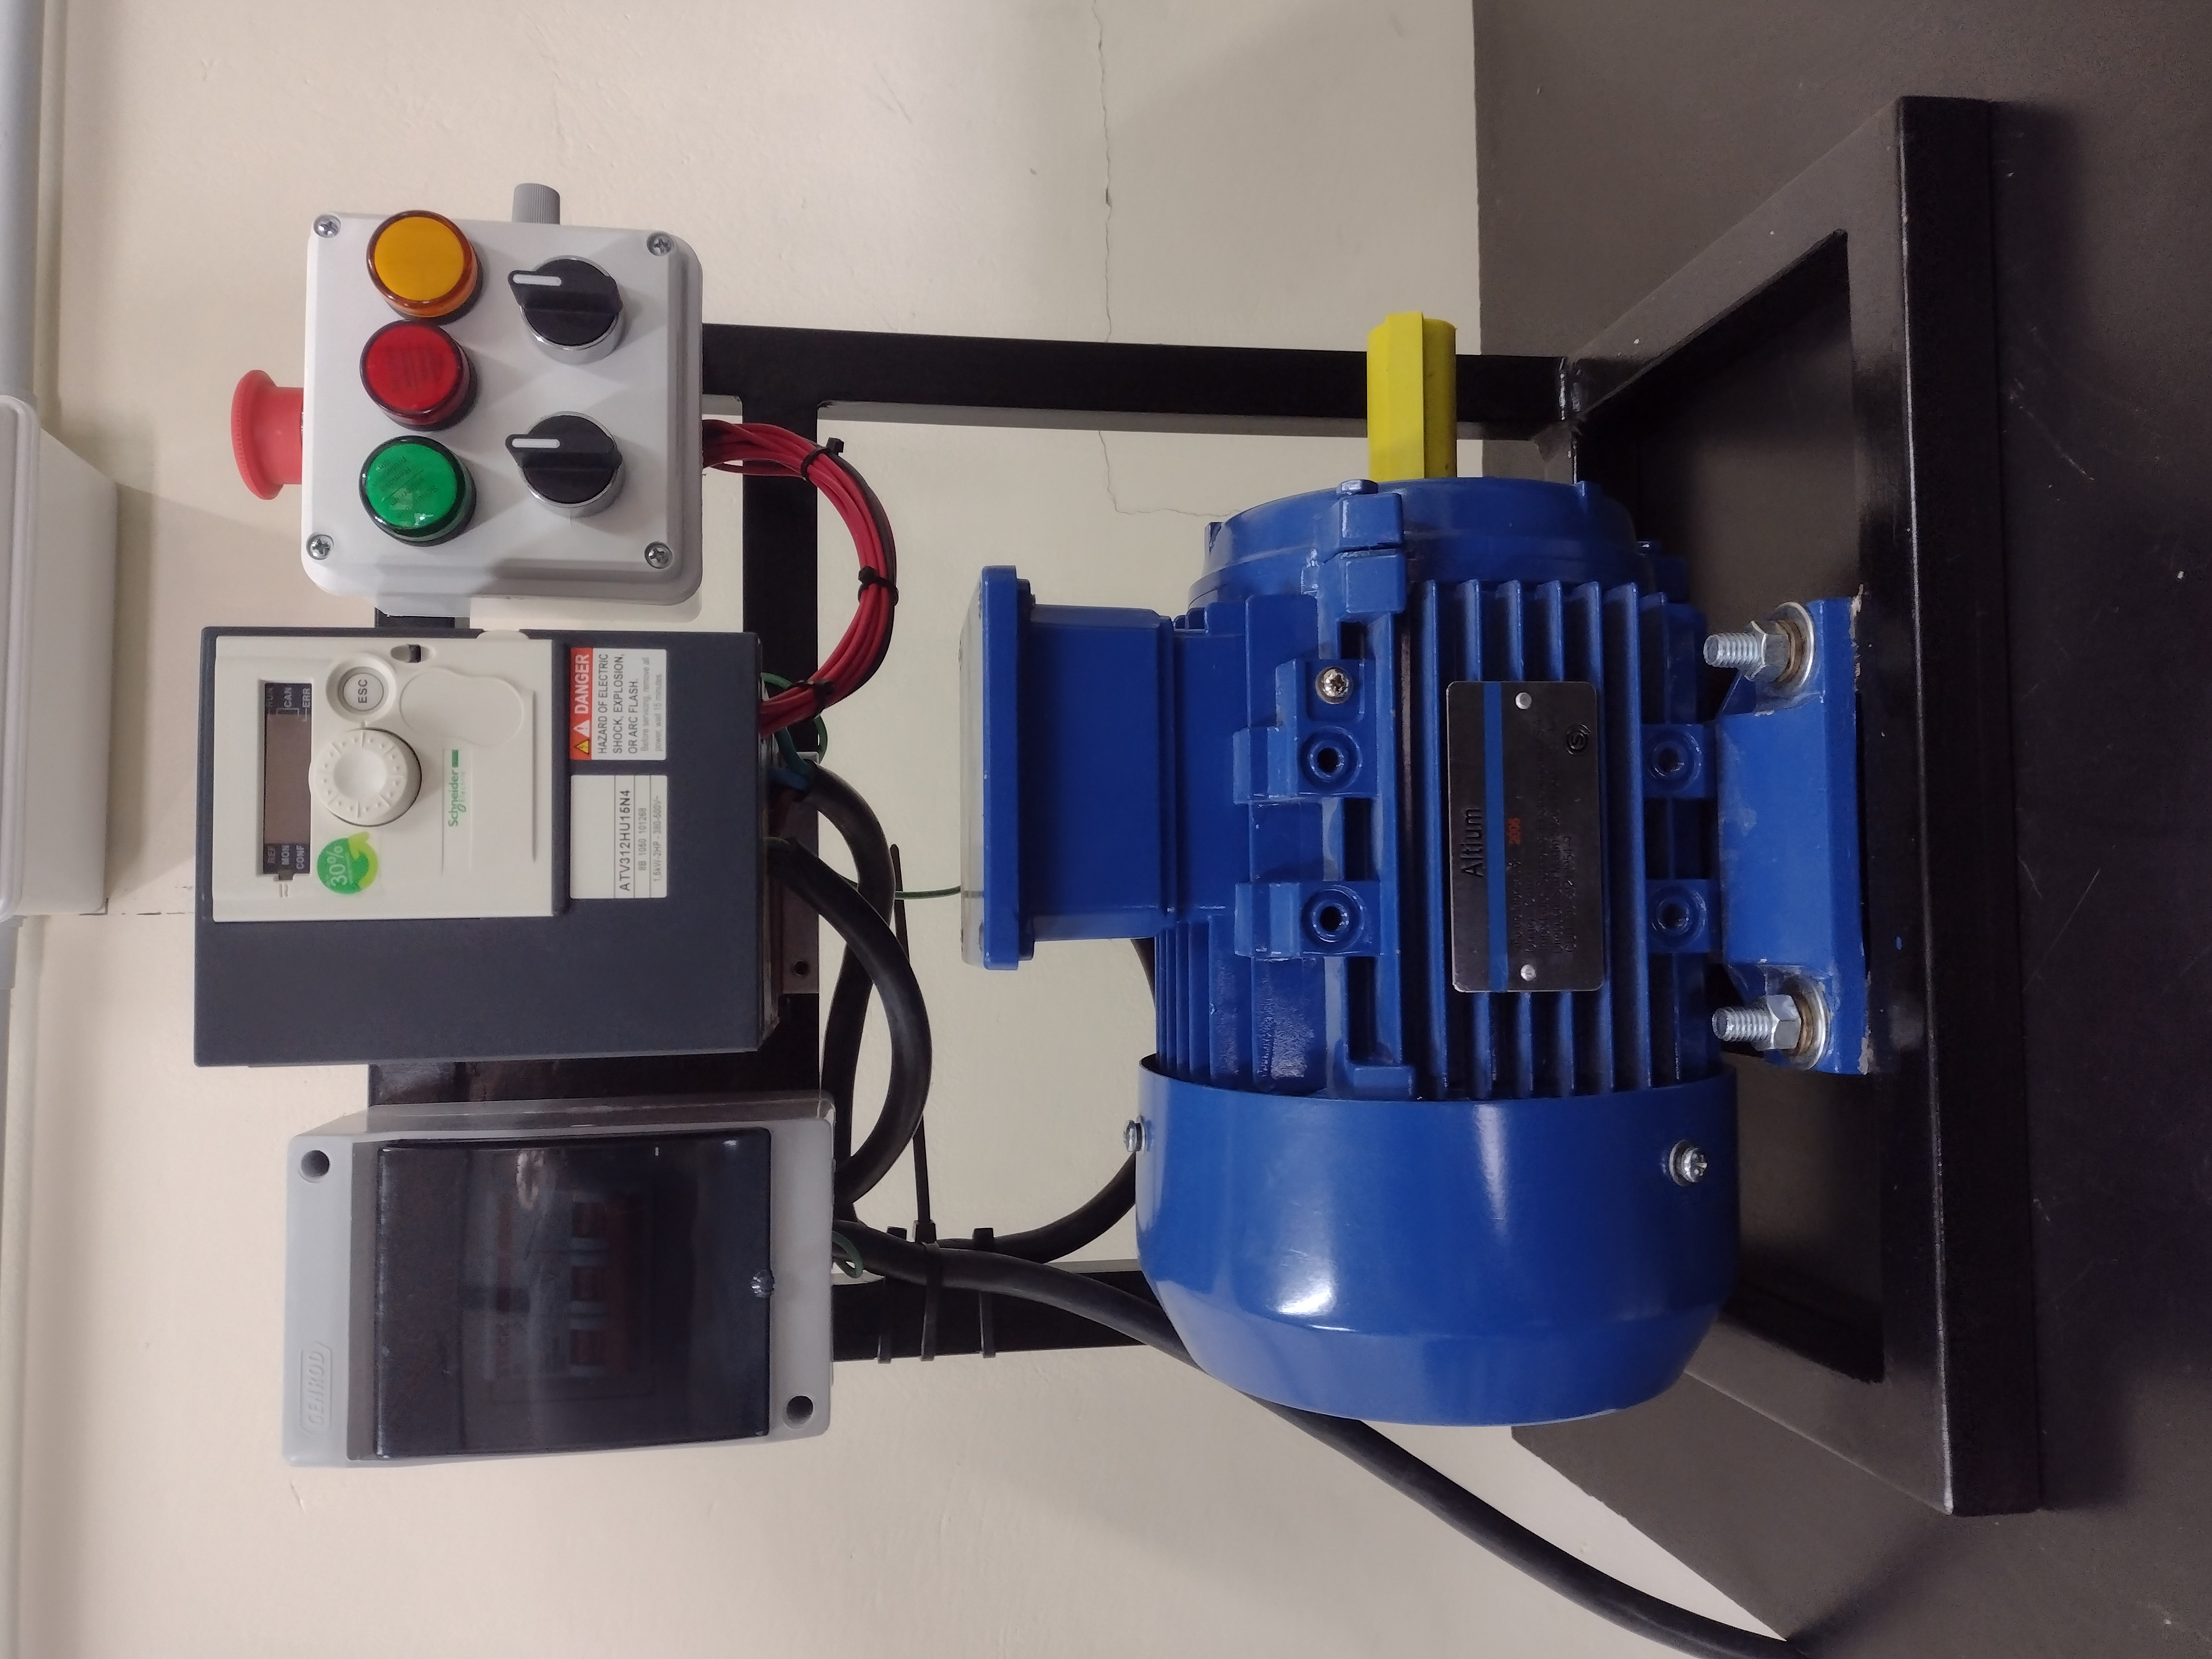
\includegraphics[angle=-90,width=70mm]{banc1 (1)}}
	\subfigure[]{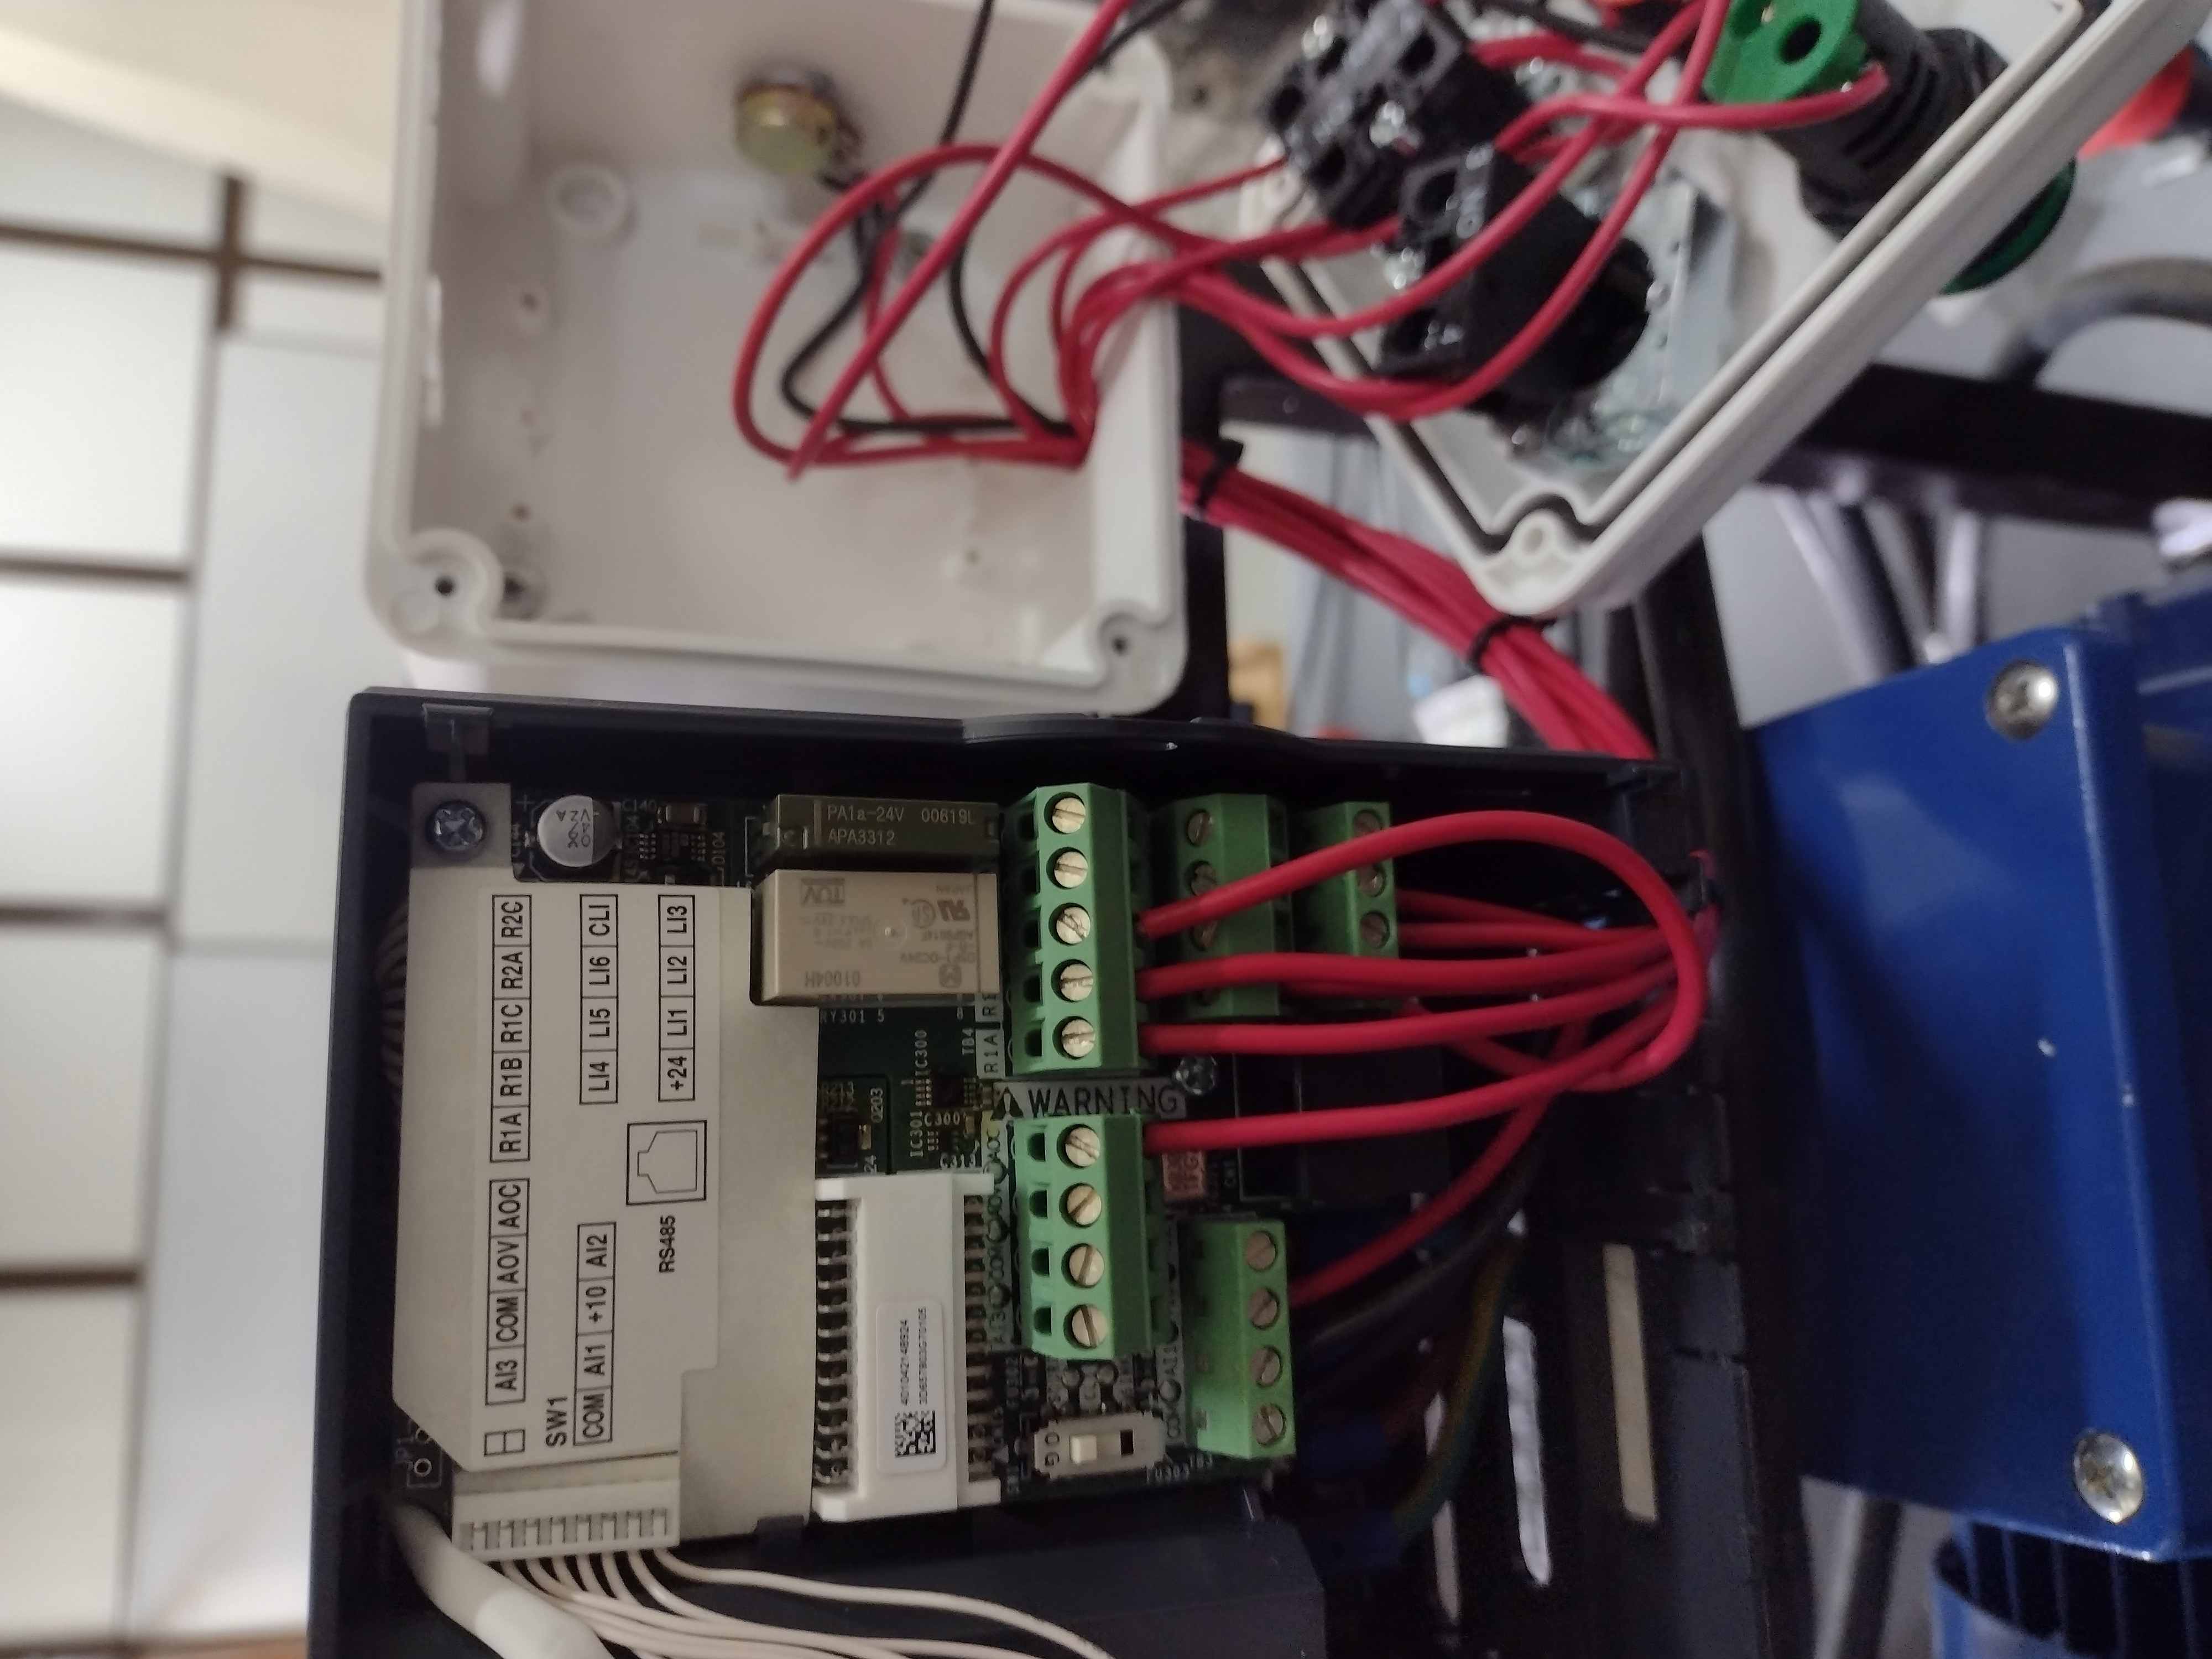
\includegraphics[angle=-90,width=70mm]{images/banc1 (2)}}
	\caption{Banco de pruebas} \label{fig:banco}
\end{figure}

\subsubsection{Transmisor de presión}
Para este proyecto se utilizan dos transmisores de presión de montaje en línea modelo EJA530E (Figura \ref{fig:transd}.a).\\
Las características del transmisor son:
\begin{itemize}
	\item Precisión: ±0,055\% 
	\item Fiabilidad: ±0,1\% (estabilidad por 10 años)
	\item Tiempo de respuesta: 90mseg.
	\item Lazo de corriente de 4-20mA
	\item Se puede configurar en la unidad necesaria, en este caso mbar.
\end{itemize}


\subsubsection{Sensor de caudal}
Se utilizó un sensor de caudal (Figura \ref{fig:transd}.b) con rotor a paleta de las siguientes características:
\begin{itemize}
	\item Rango de caudal: 2- 60 l/min
	\item Máxima presión de agua: 1,75MPa
	\item Conversión de caudal: aprox 477pulsos/L $\pm$ 10\%
\end{itemize}


\begin{figure}[htbp]
	\centering
	\subfigure[Transmisor de presión]{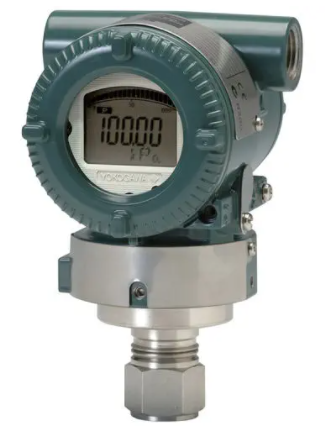
\includegraphics[height=40mm]{tran_pre.png}}
	\subfigure[Sensor de caudal]{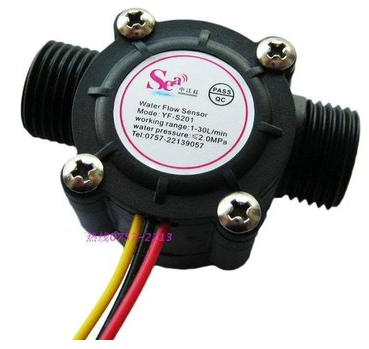
\includegraphics[height=40mm]{sens_pre.png}}
	\caption{Transmisores} \label{fig:transd}
\end{figure}





\subsection{Diagrama}
La figura \ref{fig:diag} corresponde al diagrama P\&ID realizado en base al banco de pruebas dónde se observa los respectivos elementos, sus nombres y las conexiones eléctricas, hidráulicas y mecánicas. En el Anexo \ref{anexopid} se encuentra la imagen con mayor tamaño.
 Para la nomenclatura de los instrumentos utilizados se empleó las normas ISA-S5.1 \cite{ISA}. 

\begin{figure}[htb]
	\centering
	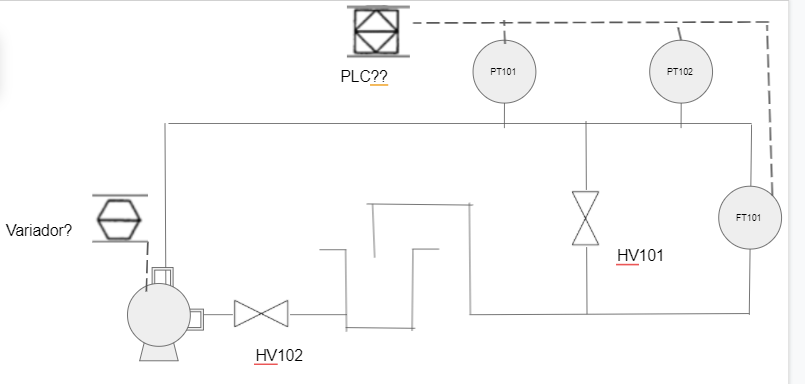
\includegraphics[width=1\linewidth]{diag.png}
	\captionof{figure}{Diagrama p\&id}
	\label{fig:diag}
\end{figure}

\begin{comment}
\subsection{Presupuesto}

%\url{https://docs.google.com/spreadsheets/d/1mFoNvgJXUdL2bNnspaBJ_wS5fFA1y1c8fTO9Rfod7H0/edit#gid=0}   https://articulo.mercadolibre.com.ar/MLA-1138428193-plc-schneider-m340-_JM#position=4&search_layout=stack&type=item&tracking_id=b8eec422-f1df-4784-a273-ea993949357f
Se realizó un presupuesto (Tabla \ref{tab:presu}) estimativo de lo gastado y lo que se hubiese gastado a lo largo del proyecto, este valor final corresponde al mes de enero 2022 y no se tiene en cuenta la bomba que era de descarte, la mano de obra ni el tiempo de programación requerido.
\begin{table}[h!]
\centering
\caption{Presupuesto}
\label{tab:presu}
\begin{tabular}{|l|r|r|r|}
\hline
\multicolumn{1}{|c|}{\textit{\textbf{Elemento}}} & \multicolumn{1}{c|}{\textit{\textbf{Cantidad}}} & \multicolumn{1}{c|}{\textit{\textbf{Valor unitario}}} & \multicolumn{1}{c|}{\textit{\textbf{Valor total}}} \\ \hline
Antióxido 1L & 0.33 & 798.9 & 266.3 \\ \hline
Disco corte & 0.33 & 325.8 & 108.6 \\ \hline
Bulones 3/8 x 11/2 & 0.33 & 64.2 & 21.4 \\ \hline
Tuercas 3/8 & 0.33 & 119.5 & 39.83 \\ \hline
Arandelas 3/8 & 0.33 & 51.8 & 17.27 \\ \hline
Caño estructural 25x25mm & 0.33 & 3140 & 1046.67 \\ \hline
Planchuela & 0.33 & 690.06 & 230.02 \\ \hline
Caja p/termica & 1 & 448.57 & 448.57 \\ \hline
Térmica serie 3P 10A & 1 & 1069.9 & 1069.9 \\ \hline
Señal luminosa roja 24V & 1 & 325 & 325 \\ \hline
Señal luminosa verde 24V & 1 & 326 & 326 \\ \hline
Señal luminosa amarilla 24V & 1 & 326 & 326 \\ \hline
Selectora 3 puntos & 1 & 940.6 & 940.6 \\ \hline
Selectora 2 puntos & 1 & 688.5 & 688.5 \\ \hline
Pulsador emergencia & 1 & 773.49 & 773.49 \\ \hline
Terminal horquilla & 16 & 5.86 & 93.76 \\ \hline
Ficha industrial, macho 380V & 1 & 680 & 680 \\ \hline
Caños de termofusión 20mm & 1 & 6000 & 6000 \\ \hline
Motor ALTIUM & 1 & 33000 & 33000 \\ \hline
Variador de velocidad ALTIVAR 312 & 1 & 130000 & 130000 \\ \hline
PLC M340 & 1 & 225000 & 225000 \\ \hline
& \multicolumn{1}{l|}{} &  & \multicolumn{1}{l|}{} \\ \hline
& \multicolumn{1}{l|}{} & Total=    \$ & \multicolumn{1}{l|}{401401.91} \\ \hline
\end{tabular}
\end{table}


\end{comment}

\clearpage
\newpage